%Version 2.1 April 2023
% See section 11 of the User Manual for version history
%
%%%%%%%%%%%%%%%%%%%%%%%%%%%%%%%%%%%%%%%%%%%%%%%%%%%%%%%%%%%%%%%%%%%%%%
%%                                                                 %%
%% Please do not use \input{...} to include other tex files.       %%
%% Submit your LaTeX manuscript as one .tex document.              %%
%%                                                                 %%
%% All additional figures and files should be attached             %%
%% separately and not embedded in the \TeX\ document itself.       %%
%%                                                                 %%
%%%%%%%%%%%%%%%%%%%%%%%%%%%%%%%%%%%%%%%%%%%%%%%%%%%%%%%%%%%%%%%%%%%%%

\documentclass[sn-apa,referee,pdflatex]{sn-jnl}

%%%% Standard Packages
%%<additional latex packages if required can be included here>

\usepackage{graphicx}%
\usepackage{multirow}%
\usepackage{amsmath,amssymb,amsfonts}%
\usepackage{amsthm}%
\usepackage{mathrsfs}%
\usepackage[title]{appendix}%
\usepackage{xcolor}%
\usepackage{textcomp}%
\usepackage{manyfoot}%
\usepackage{booktabs}%
\usepackage{algorithm}%
\usepackage{algorithmicx}%
\usepackage{algpseudocode}%
\usepackage{listings}%
%%%%

%%%%%=============================================================================%%%%
%%%%  Remarks: This template is provided to aid authors with the preparation
%%%%  of original research articles intended for submission to journals published
%%%%  by Springer Nature. The guidance has been prepared in partnership with
%%%%  production teams to conform to Springer Nature technical requirements.
%%%%  Editorial and presentation requirements differ among journal portfolios and
%%%%  research disciplines. You may find sections in this template are irrelevant
%%%%  to your work and are empowered to omit any such section if allowed by the
%%%%  journal you intend to submit to. The submission guidelines and policies
%%%%  of the journal take precedence. A detailed User Manual is available in the
%%%%  template package for technical guidance.
%%%%%=============================================================================%%%%




\raggedbottom




% tightlist command for lists without linebreak
\providecommand{\tightlist}{%
  \setlength{\itemsep}{0pt}\setlength{\parskip}{0pt}}





\begin{document}


\title[]{Estimating the socio-environmental impacts of car substitution
by bicycle and public transit using open tools}

%%=============================================================%%
%% Prefix	-> \pfx{Dr}
%% GivenName	-> \fnm{Joergen W.}
%% Particle	-> \spfx{van der} -> surname prefix
%% FamilyName	-> \sur{Ploeg}
%% Suffix	-> \sfx{IV}
%% NatureName	-> \tanm{Poet Laureate} -> Title after name
%% Degrees	-> \dgr{MSc, PhD}
%% \author*[1,2]{\pfx{Dr} \fnm{Joergen W.} \spfx{van der} \sur{Ploeg} \sfx{IV} \tanm{Poet Laureate}
%%                 \dgr{MSc, PhD}}\email{iauthor@gmail.com}
%%=============================================================%%

\author*[1]{\fnm{Rosa} \sur{Félix} }\email{\href{mailto:rosamfelix@tecnico.ulisboa.pt}{\nolinkurl{rosamfelix@tecnico.ulisboa.pt}}}

\author[1]{\fnm{Filipe} \sur{Moura} }\email{\href{mailto:fmoura@tecnico.ulisboa.pt}{\nolinkurl{fmoura@tecnico.ulisboa.pt}}}

\author[2]{\fnm{Robin} \sur{Lovelace} }\email{\href{mailto:r.lovelace@leeds.ac.uk}{\nolinkurl{r.lovelace@leeds.ac.uk}}}



  \affil*[1]{\orgdiv{CERIS - Instituto Superior
Técnico}, \orgname{University of
Lisbon}, \orgaddress{\city{Lisbon}, \country{Portugal}, \postcode{1049-001}, \street{Av
Rovisco Pais 1}}}
  \affil[2]{\orgdiv{Institute for Transport
Studies}, \orgname{University of
Leeds}, \orgaddress{\city{Leeds}, \country{United
Kingdom}, \postcode{LS2 9JT}, \street{34-40 University Rd}}}

\abstract{In metropolitan areas, car trips can be replaced by a
combination of public transit and cycling for the first-and-last mile.
This approach requires interventions to make cycling more appealing, and
the resulting public investments can have significant social and
environmental benefits. This paper focuses on estimating the potential
for cycling + PT as a substitute for car trips in the Lisbon
metropolitan area and assessing its socio-environmental impacts using
open data and open source tools.

To achieve the cycling targets set by the Portuguese cycling strategy,
the Department of Transport introduced \emph{biclaR}, a decision support
tool that facilitates the design and development of a metropolitan
cycling network. A scenario of intermodality introduced, and its
socio-environmental impacts were assessed using the \emph{HEAT for
Cycling} and the \emph{HEAT as a Service} tools. Additionally, we
estimated the impacts of shifting car trips to PT and monetize them with
the EU Guide to cost-benefit analysis.

The results indicate that 20\% of the current trips can be made with the
bicycle + PT combination, with an additional 12\% of PT trips being
potentially replaced. Shifting to cycling for the first-and-last mile
can reduce annual CO2eq emissions by 6,000 to 15,000 tons/day, and the
10-year socio-environmental benefits account for €230 to €590 million,
depending on the cycling targets. For the PT leg, the transfer from car
results in the avoidance of 8,500 to 20,800 tons of CO2eq emissions per
year.

The provided information on socio-economic benefits can support
policymakers in prioritizing interventions to reduce the reliance on
individual motorized transportation and effectively communicate their
decisions.}

\keywords{Active transport, Intermodality, First and last mile, Health
economic assessment, Environmental impacts, Open data and methods}



\maketitle

\hypertarget{sec1}{%
\section{Introduction}\label{sec1}}

The Introduction section should explain the background to the study, its
aims, a summary of the existing literature and why this study was
necessary.

In metropolitan areas, car trips can be replaced by a combination of
public transit (PT) and cycling for the first-and-last mile. This
approach requires interventions and programs to make bicycling more
appealing, and the resulting public investments can have significant
social and environmental benefits. This paper focuses on estimating the
potential for cycling + PT as a substitute for car trips in the Lisbon
metropolitan area (LMA) and assessing its socio-environmental impacts
using open data and open source tools.

According to the latest mobility survey conducted in 2018, the LMA
registered a total of 5.3 million daily trips, with only 0.5\% by
bicycle. Car modal share is 58.4\%, while PT accounts for 15.5\%. To
achieve the cycling targets set by the Portuguese national cycling
strategy for 2025 and 2030 (4\% and 10\%, respectively), the Department
of Transport introduced biclaR, a decision support tool that facilitates
the design and development of a metropolitan cycling network.

The intermodality scenario considers trips that can combine PT and
cycling for the first-and-last legs. Conservatively, we considered the
sum of first-and-last legs up to 5 km. Furthermore, we restricted PT use
to unimodal trips without transfers (although they can be included in
future modeling). Finally, we only included PT modes that can
practically accommodate bicycles, such as trains, ferries, trams, and
intermunicipal bus lines with bike racks (Figure 1).

To obtain reliable results, we used the OpenStreetMap road network and
GTFS data. The r5r R package estimated the trip duration and distance
for both the original modes and the bicycle + PT combination, while the
od jittering R package estimated the OD locations based on a
centroid-based OD matrix.

Socio-environmental impacts were assessed using the HEAT for Cycling and
the HEAT as a Service tools, from the WHO. Additionally, we estimate the
impacts of shifting car trips to PT for the second leg of the journey
with EMEP/EEA's COPERT methodology and monetize them with the EU Guide
to cost-benefit analysis.

The results indicate that 20\% of the current trips can be made with the
bicycle + PT combination, with an additional 12\% of PT trips being
potentially replaced. Shifting to cycling for the first-and-last mile
can reduce annual CO2eq emissions by 6,000 to 15,000 tons/day, and the
10-year socio-environmental benefits account for €230 to €590 million,
depending on the cycling targets. For the PT leg, the transfer from car
results in the avoidance of 8,500 to 20,800 tons of CO2eq emissions per
year, or €1.4 to €3.5 million over 10 years, with trains offering the
greatest potential for substitution (88\%).

By making the research process publicly accessible in a code repository,
this study enables the replication of similar estimates for
socio-environmental impacts resulting from a modal shift from cars to
bicycles + PT in other metropolitan areas. The provided information on
socio-economic benefits can support policymakers in prioritizing
interventions to reduce the reliance on individual motorized
transportation and effectively communicate their decisions.

The Introduction section, of referenced text \citet{bib1} expands on the
background of the work (some overlap with the Abstract is acceptable).
The introduction should not include subheadings.

Springer Nature does not impose a strict layout as standard however
authors are advised to check the individual requirements for the journal
they are planning to submit to as there may be journal-level
preferences. When preparing your text please also be aware that some
stylistic choices are not supported in full text XML (publication
version), including coloured font. These will not be replicated in the
typeset article if it is accepted.

\hypertarget{sec2}{%
\section{Methods}\label{sec2}}

The methods section should include:

\begin{itemize}
\tightlist
\item
  the aim, design and setting of the study
\item
  the characteristics of participants or description of materials
\item
  a clear description of all processes and methodologies employed.
  Generic names should generally be used. When proprietary * brands are
  used in research, include the brand names in parentheses
\item
  the type of statistical analysis used, including a power calculation
  if appropriate
\item
  studies involving human participants, data or tissue or animals must
  include statement on ethics approval and consent
\end{itemize}

\begin{figure}
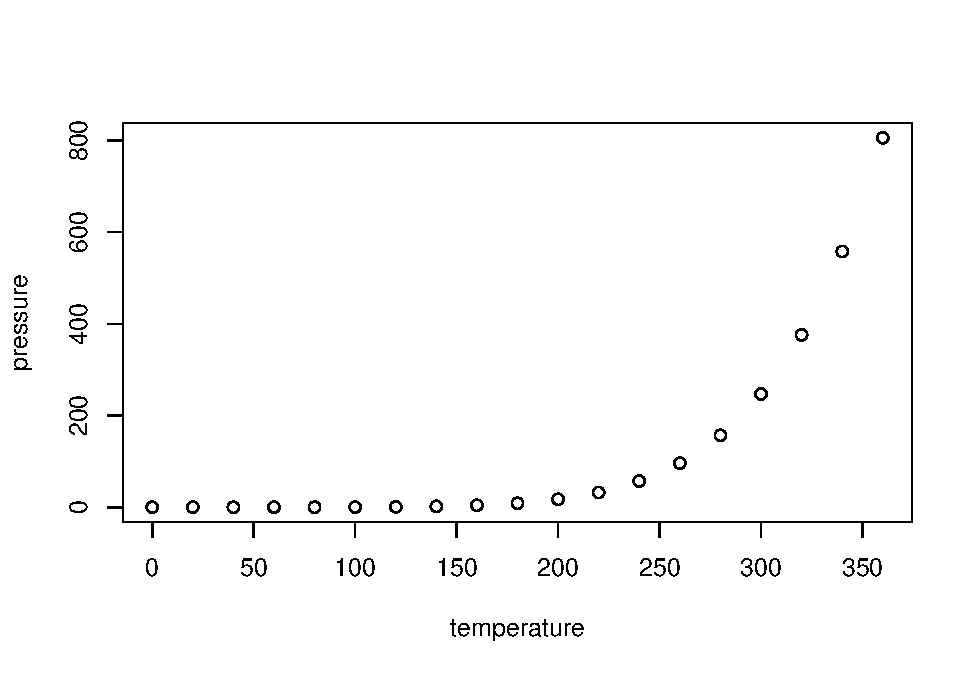
\includegraphics{PaperTRA_files/figure-latex/fig1-1} \caption{This is an example of a caption}\label{fig:fig1}
\end{figure}

\hypertarget{sec11}{%
\section{Results and Discussion}\label{sec11}}

Topical subheadings are allowed. Authors must ensure that their Methods
section includes adequate experimental and characterization data
necessary for others in the field to reproduce their work. Authors are
encouraged to include RIIDs where appropriate.

\textbf{Ethical approval declarations} (only required where applicable)
Any article reporting experiment/s carried out on
(i)\textasciitilde live vertebrate (or higher invertebrates),
(ii)\textasciitilde humans or (iii)\textasciitilde human samples must
include an unambiguous statement within the methods section that meets
the following requirements:

\begin{enumerate}
\def\labelenumi{\arabic{enumi}.}
\item
  Approval: a statement which confirms that all experimental protocols
  were approved by a named institutional and/or licensing committee.
  Please identify the approving body in the methods section
\item
  Accordance: a statement explicitly saying that the methods were
  carried out in accordance with the relevant guidelines and regulations
\item
  Informed consent (for experiments involving humans or human tissue
  samples): include a statement confirming that informed consent was
  obtained from all participants and/or their legal guardian/s
\end{enumerate}

If your manuscript includes potentially identifying patient/participant
information, or if it describes human transplantation research, or if it
reports results of a clinical trial then additional information will be
required. Please visit
(\url{https://www.nature.com/nature-research/editorial-policies}) for
Nature Portfolio journals,
(\url{https://www.springer.com/gp/authors-editors/journal-author/journal-author-helpdesk/publishing-ethics/14214})
for Springer Nature journals, or
(\url{https://www.biomedcentral.com/getpublished/editorial-policies/\#ethics+and+consent})
for BMC.

\hypertarget{sec13}{%
\section{Conclusion}\label{sec13}}

This should state clearly the main conclusions and provide an
explanation of the importance and relevance of the study to the field.

Conclusions may be used to restate your hypothesis or research question,
restate your major findings, explain the relevance and the added value
of your work, highlight any limitations of your study, describe future
directions for research and recommendations.

In some disciplines use of Discussion or `Conclusion' is
interchangeable. It is not mandatory to use both. Please refer to
Journal-level guidance for any specific requirements.

\backmatter

\bmhead{Acknowledgments}

Acknowledgments are not compulsory. Where included they should be brief.
Grant or contribution numbers may be acknowledged.

Please refer to Journal-level guidance for any specific requirements.

\hypertarget{declarations}{%
\section*{Declarations}\label{declarations}}
\addcontentsline{toc}{section}{Declarations}

Some journals require declarations to be submitted in a standardised
format. Please check the Instructions for Authors of the journal to
which you are submitting to see if you need to complete this section. If
yes, your manuscript must contain the following sections under the
heading `Declarations':

\begin{itemize}
\tightlist
\item
  Funding
\item
  Conflict of interest/Competing interests (check journal-specific
  guidelines for which heading to use)
\item
  Ethics approval
\item
  Consent to participate
\item
  Consent for publication
\item
  Availability of data and materials
\item
  Code availability
\item
  Authors' contributions
\end{itemize}

\noindent If any of the sections are not relevant to your manuscript,
please include the heading and write `Not applicable' for that section.

\renewcommand\refname{References}
\bibliography{bibliography.bib}


\end{document}
